% (C) Anders Kofod-Petersen
\documentclass[a4paper,norsk,oneside]{article}
\usepackage[norsk]{babel}						% Correct English hyphenation
\usepackage[utf8]{inputenc}						% Allow for non-English letters
\usepackage{graphicx}							% To include graphics
%\usepackage{natbib}								% Correct citations
%\usepackage{fancyheadings}						% Nice header and footer
\usepackage[linktocpage,colorlinks]{hyperref}			% PDF hyperlink
\usepackage{geometry} 							% Better geometry
%\usepackage[center]					% For cropping documents
\usepackage{url}
\usepackage{float}
% B5 (uncomment to convert to B5 format)
 \geometry{b5paper}

% Author
% Fill in here, and use commands in the text. 
\newcommand{\thesisAuthor}{Sania Ahktar\\Andreas Hagen\\Øystein Heimark\\Steffen Henriksen\\Eirik Hjelle\\Odd Andreas Sørsæther}
\newcommand{\thesisTitle}{Det intelligente transportsystem }
\newcommand{\thesisType}{Prosessrapport - Eksperter i Team - Geokomai}
\newcommand{\thesisDate}{Vår 2013}

% PDF info
\hypersetup{pdfauthor={\thesisAuthor}}
\hypersetup{pdftitle={\thesisTitle}}
\hypersetup{pdfsubject={\thesisType}}
\hypersetup{linkcolor=black}
\hypersetup{citecolor=black}
\hypersetup{urlcolor=black}

%Fancy headings
%\pagestyle{fancy}
%\pagestyle{fancyplain}
%\renewcommand{\chaptermark}[1]{\markboth{#1}{}}
%\renewcommand{\sectionmark}[1]{\markright{#1}{}}
%\lhead[\fancyplain{}{\thepage}]{\fancyplain{}{\let\uppercase\relax\leftmark}}
%\rhead[\fancyplain{}{\let\uppercase\relax\rightmark}]{\fancyplain{}{\thepage}}
%\chead[\fancyplain{}{}]{\fancyplain{}{}}
%\lfoot[\fancyplain{}{}]{\fancyplain{}{}}
%\cfoot[\fancyplain{}{}]{\fancyplain{}{}}
%\rfoot[\fancyplain{}{}]{\fancyplain{}{}}

% Citation format
%\bibliographystyle{apalike}
%\bibpunct{[}{]}{;}{a}{,}{,}

\begin{document}

%Title page (This is generate automatically from the commands above)
\begin{titlepage}
\noindent {\large \textbf{\thesisAuthor}}
%\vspace{2cm}
\vspace{3cm}

\noindent {\Huge \thesisTitle}
\vspace{2cm}

\noindent \thesisType, \thesisDate 
\vspace{2cm}

%\noindent Artificial Intelligence Group\\ Department of Computer and Information Science\\ Faculty of Information Technology, Mathematics and Electrical Engineering\\

\vfill
\begin{center}

\includegraphics[width=3cm]{figs/NTNUlogo.pdf}
\end{center}
\end{titlepage}

\thispagestyle{empty}

\cleardoublepage

%\frontmatter

%\section*{Innledning}
%
%I dag finnes det en rekke applikasjoner og tilgjengelig informasjon relatert til vei, veiforhold, navigasjon, kart, trafikkmeldinger og lignende. Tjenesten Google Maps er nok for mange et kjent fenomen som er en web-basert applikasjon for kart og navigasjon. Det er også flere kilder som tilbyr informasjon i forbindelse med både trafikkmeldinger og værdata, som for eksempel vegvesenet og yr.no. Alt dette er viktige faktorer for å kunne avgjøre om en reiserute er trygg og effektiv, og det er nettopp dette vi vil belyse i denne oppgaven. Prosjektet vårt går ut på å samordne eksisterende kilder til sanntidsinformasjon til et integrert intelligent system som kan ta beslutninger om hvilke reiseruter som er tryggest og mest effektive for veiferdsel. Den store utfordringen vil være å samordne informasjon og data fra flere forskjellige kilder, som igjen kan danne et grunnlag for å presentere dette på en enkel plattform.

\section*{Forord}



\vspace{1cm}

Denne rapporten er en prosessrapport som er utarbeidet i emnet “Eksperter i Team”. Emnet er et obligatorisk fag på NTNU, og er for studenter som går fjerde klasse ved et masterprogram. Hensikten med “Eksperter i Team” er å lære studenter å samarbeide på tvers av studieprogram, og er opprettet etter ønske fra det norske næringslivet.

Vi vil gjerne takke landsbyleder, Pauline Haddow, for veiledning og tilbakmeldinger, samt fasiliteringen fra Eivind Myklebust Lindseth og Edel Gustavsen Holand, som har har hjulpet oss med blant annet nyttige øvelser relatert til prosess og refleksjon. 





\vfill

%\hfil
\noindent
\thesisAuthor

\hfill Trondheim, \today
\cleardoublepage

\section*{Sammendrag} 
Prosessrapporten er en del av faget, Eksperter i Team ved NTNU. Det er sluttdokumentet hvor gruppens sammensetning, motivasjon og utvikling blir presentert med refleksjoner og analyser av hendelser. Den gjenspeiler den personlige utvikling hver av oss har vært gjennom og gruppens utvikling i løpet av vårsemesteret 2013 for gruppen Geokomai. 

Utfordringer underveis i forming-, storming- og normingsfasene kan sies at ha vært lite konfliktfylt. Grunnene for dette er ulike, men kan forklares med at samarbeidsavtalen mellom medlemmene har gjort at samtlige studenter var inneforstått med krav til gjensidig respekt og arbeidsoppgaver. Gruppen ble etter hvert flinkere til å teste sine antakelser og har brukt mye tid til diskusjon rundt forskjellige problemstillinger. Dette har medlemmene jobbet aktivt med for å opprettholde en god dialog mellom seg selv og andre.Gruppen har beveget seg mellom kategoriene pseudogruppe, tradisjonell gruppe og effektiv gruppe. Det har ikke vært en lineær progresjon. Gruppen har ved forskjellige faser og forskjellige problemstillinger tatt ulike former innen gruppedynamikk. 

Refleksjoner rundt faget blir også presentert i denne rapporten. Fasiliteringen har vært viktig for innspill og forståelse av vårt samarbeid. Medlemmene har blandede følelser om hvor godt de ulike fasiliteringsmetodene har fungert gjennom semesteret, men har i etterkant reflektert og forstått hvor viktig det er for å bedre dynamikken og samarbeidet i gruppen. Sosiogram og SPGR-test var de verktøyene medlemmene fikk mest igjen for i faget.

\clearpage
\tableofcontents

\clearpage

\section{Innledning}
Gruppen som har skrevet denne rapporten heter “Geokomai”. Tanken bak navnet er tverrfaglighet, hvor vi har slått sammen ordene geomatikk, geofag,  kommunikasjonsteknologi og AI (artificial intelligence). Flertallet av studentene i denne gruppen har fordypning innen Informasjonsteknologi og data, og det har dermed vært ekstra viktig å ha hensyn til vedkommende som har teknisk geofag som sitt område.

Dette emnet er delt i to, hvor hver del spiller en like stor rolle. Den ene delen går ut på at gruppen sammen skal klare å definere en problemstilling relatert til sin landsby, som skal kunne danne et utgangspunkt for en prosjektoppgave. Den andre delen omhandler det å kunne lære seg selv å kjenne i et tverrfaglig samarbeid. Refleksjon er et viktig nøkkelord i denne prosessen, og det har blitt brukt og analysert under hver eneste landsbydag. Ulike øvelser, personlig logg og gruppelogg har hjulpet oss med å reflektere over oss selv som enkeltindivider og gruppen som helhet. 

Denne rapporten omhandler kun prosessdelen. Den skal kunne gi leseren et innblikk i hvordan Geokomai har fungert i sitt samarbeid, hva hver enkelt har fått ut av å jobbe på denne måten, og sist men ikke minst hvilke utfordringer som har dukket opp. Både de personlige loggene, samt de grupperelalterte er nøye analysert og vært til stor hjelp for å kunne utarbeide en prosessrapport. I tillegg til dette har kompendiet og presentasjoner i emnet hjulpet oss med å ta i bruk relevant teori.

\clearpage

\section{Presentasjon av gruppen}
\begin{figure}[H]
\centering
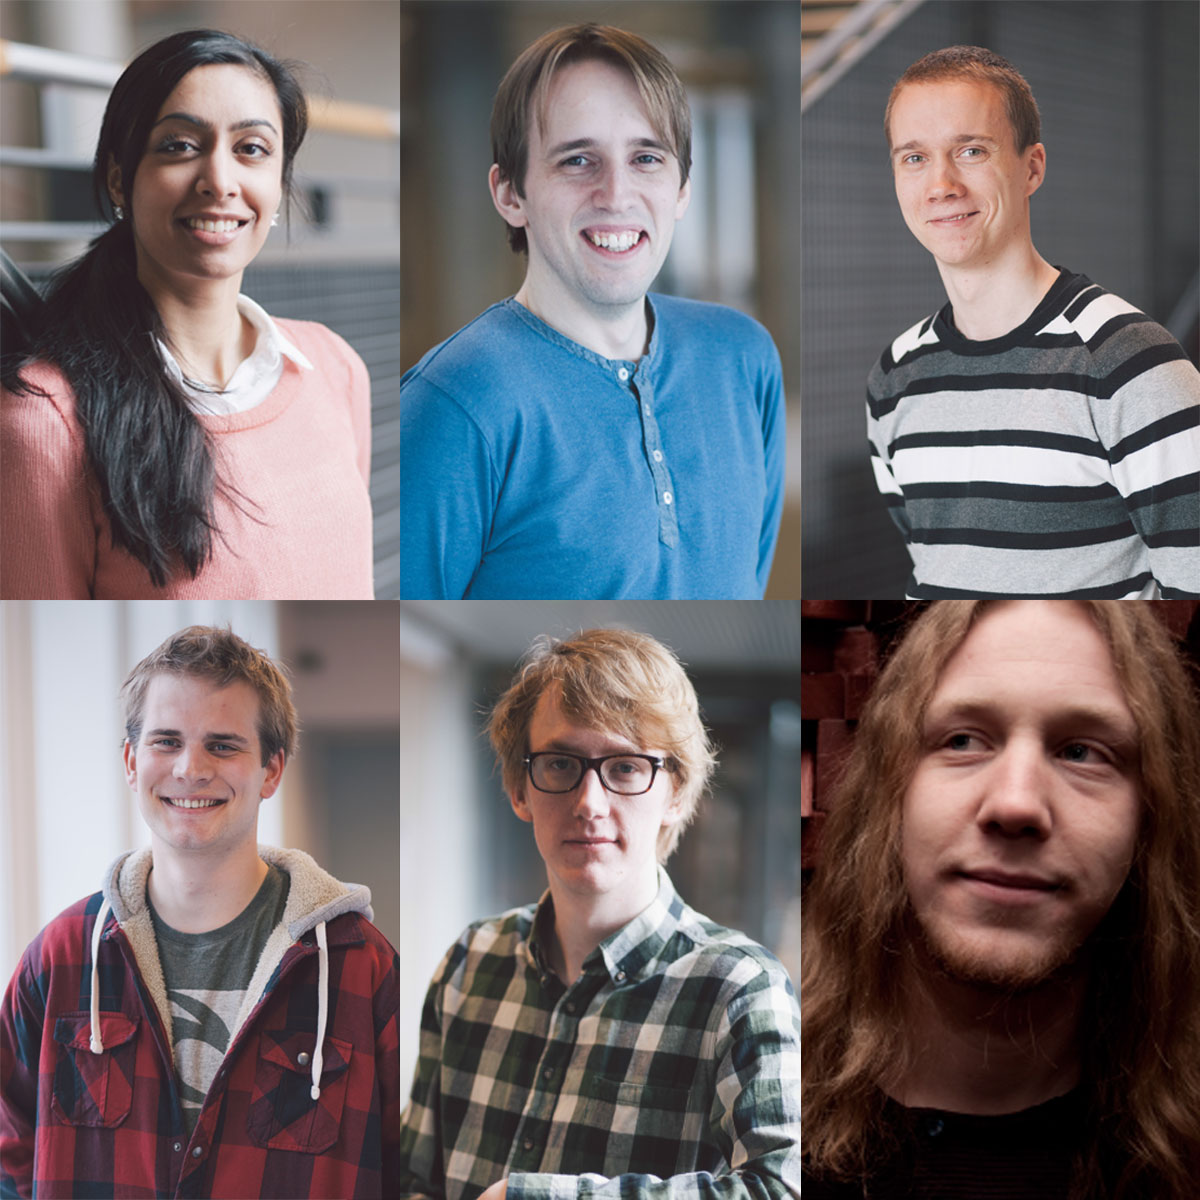
\includegraphics[scale=0.25]{figs/gruppebildegeokomai}
\label{gmaps1}
\caption{Fra øv. med klokken: Sania, Odd, Øystein, Andreas, Steffen, Eirik}
\end{figure}


\textbf{Eirik Hjelle}\\
Eirik har bakgrunn fra Teknisk Geofag med en fordypning rettet mot mineralressurs og teknologi. Han liker utfordringer og er ikke redd for å dumme seg ut. Prater ofte om løst og fast og kan til tider spore litt av. Han liker konfrontasjoner når det er han som tar opp problemer. Det å bli sett og hørt, for deretter å få tilbakemeldinger er noe han setter pris på. Han beskriver seg selv som “en som liker å sparke oppover” og kan i samtaler velge å ta motsatt side av hva han egentlig står for, bare for å få liv i en debatt. Han er en aktiv person med mange forskjellige hobbyer, som til tider kan gå utover skolehverdagen. En typisk personlighet som har “for mange baller i luften.”   \\
\newline
\newline
\textbf{Sania Akhtar}\\
Sania går Kommunikasjonsteknologi hvor hun fordyper seg i Teleøkonomi. Hun er veldig opptatt av planlegging og struktur og foretrekker ikke å gjøre ting i siste liten. Utenom dette oppfattes hun som en blid og samarbeidvillig person. På fritiden liker hun å trene og spille squash. Og sist men ikke minst har hun en genuin interesse for baking. 	
\newline
\newline
\textbf{Steffen Pøhner Henriksen}\\
Steffen går Ingeniørvitenskap og IKT med spesialisering innen geomatikk. Han er interessert i programmering og har mange fag med dette som tema. Han kan sees på som en datastudent med spesialisering innen geografiske applikasjoner. Steffen er utadvent og ivrig. Interessen for fotografi er altoppslukende, og han bruker mye tid på Fotogjengen på Studentersamfundet i Trondhjem.
\newline
\newline
\textbf{Odd Andreas Sørsæther}\\
En informatikkstudent som har valgt studieretningen Intelligente systemer, og er en av tre gruppemedlemmer som fordyper seg i kunstig intelligens. Odd Andreas kommer fra et ingeniørstudium på Høgskolen i Sør-Trøndelag og har vært nødt til å tilpasse seg NTNU-miljøet på kort tid. Han liker å bidra til en positiv tone i gruppen og oppfattes derfor ofte som en glad og fornøyd person. Han er en perfeksjonist som ofte blir handlingslammet dersom han ikke er fornøyd med arbeid han har gjort.
\newline
\newline
\textbf{Øystein Heimark}\\
Øystein går på linjen Datateknikk og spesialiserer seg innen kunstig intelligens. Han er en strukturert og målrettet person som liker utfordringer. Han er en selvstendig person og som av og til kan oppfattes som litt tilbaketrukket. På fritiden er han en aktiv person som har stor interesse for sport generelt og spesielt fotball. Han driver i tillegg eget IT- selskap utenfor skolen sammen med flere av studiekameratene.
\newline
\newline
\textbf{Andreas Hagen}\\
Andreas går på linjen Datateknikk og spesialiserer seg innen kunstig intelligens. Han har vært meget engasjert i linjeforeningsarbeid hvor han har vært redaktør i linjeforeningsavisen og vært med på å starte opp linjeforeningens eget husband. Han jobber i studentgruppen AltUnd som jobber for å forbedre undervisningstilbudet på NTNU. På fritiden er han meget aktiv innen musikk.


\section{Samarbeidsavtalen}
For å konkretisere forventningene medlemmene av gruppen hadde til hverandre ble det utarbeidet et samarbeidsavtale som samtlige skulle undertegne. Samarbeidsavtalen skulle klart og tydelig føre opp hvilket ansvar alle i gruppen hadde og hvilke konsekvenser det ville få hvis noen i gruppen ikke utførte det ansvaret de var ført opp til. Gruppen så det som viktig å sørge for at sanksjoner ikke utelukkende skulle oppleves som negativt og demoraliserende, men at det burde være en avstraffelse med en grad av positiv assosiasjon. Det ble derfor bestemt at standardsanksjonen for et vanlig kontraktsbrudd skulle være å måtte bake en kake eller lignende og ta med på neste møte.

\section{Motivasjonsnivå}
En av de første temaene drøftet var motivasjonsnivået blant deltagerene. Det var konsensus om at det var viktig å etablere et felles mål for å sørge for at alle var inneforstått med hva som var forventet av dem og hva de kunne forvente av de andre medlemmene. Medlemmene i gruppen forklarte kort etter tur hva de ønsket å oppnå med prosjektet og hvor mye innsats de ønsket å legge ned i arbeidet. Det kan i ettertid påpekes at det er tydelig i en slik prosess at de med lavest motivasjonsnivå implisitt blir tvunget til å følge de med høyest motivasjonsnivå siden få på dette tidspunktet ville vært villige til å argumentere for en lavere målsetning. Det kan hevdes at dette er positivt for gruppen som helhet fordi resultatet er at alle binder seg til et høyt ambisjonsnivå. Tanken var at dette skulle hjelpe oss hvis det ble misforhold mellom hvor mye en person jobbet og hvor mye resten av gruppen mente at man skulle jobbe.
	
Etter at alle hadde lagt frem sine tanker ble dette diskutert med det formål å konkretisere ambisjonsnivået. Enkelte ville gjerne ta sikte på å ligge over en bestemt karakter, mens andre argumenterte for at det var vanskelig å sikte på en bestemt karakter. Odd Andreas opplevde det i utgangspunktet som banalt å kontraktfeste en karakter, da han ikke skjønte hvordan et slikt mål kunne oppfølges på en god måte underveis. Han innså etter hvert at samarbeidsavtalen ikke kun behøver å inneholde krav og regler, og at ambisjonsnivået skulle inkluderes for å øke motivasjonen til gruppemedlemmene. Det ble til slutt enighet om at gruppen hadde som mål å få karakter B eller høyere og dette ble senere ført inn i samarbeidsavtalen som ble utarbeidet.

\section{Utfordringer rundt tverrfaglighet}
Et av hovedmålene med “Eksperter i Team” er å gi studentene erfaring med tverrfaglig arbeid. Evnen til å kunne samarbeide med individer som har en helt annen kompetanse enn en selv er en svært nyttig erfaring å ta med seg inn i arbeidslivet. Andreas, Øystein, Odd Andreas og Sania har bakgrunn innenfor Informasjonsteknologi som er veldig relevant for EiT-landsbyen ITS. Steffen med sin Geomatikkbakgrunn, som blant annet omhandler kart, har også god kjennskap til data og IT. Eirik fra teknisk geofag har gode kunnskaper innenfor geologi med spesialisering mot mineralressursteknologi. 

Gruppen startet tidlig i formingsfasen med å kartlegge og diskutere hverandres utdanning og hva de enkelte mente de kunne tilby av kompentanse. Idémyldringen ble tidlig i satt igang. Etterhvert som tiden gikk og prosjektbeskrivelse nærmet seg ble det klart at det var dragning mot forskjellige ideer. “Gruppen startet dagen med å presentere alle ideene og diskutere kort for og i mot hvert prosjekt. Etterhvert ble det formet en positiv stemning rundt ett av prosjektene, hvor Eirik befant seg ‘litt på siden’ av ideen.” (Gruppelogg 6/02) Dette var de første gangen Eirik oppfattet i sitt fagområdet som et problem.Han følte ofte at hans kompetanse var relevant for problemstillingene som ble diskutert, men ikke fikk formidlet dette godt nok til resten av gruppen. Han skrev selv i sin personlige logg: “Jeg lurer på om vi er fanget i forskjellige ‘fagbobler’, siden de ser på min ekspertise som en utfordring, når det ikke trenger å være det.”  Her poengterer Eirik at han er redd for at han skal havne i en situasjon hvor han blir utstøtt av gruppen. Man må arbeide for å unngå og havne i situasjoner hvor faglige klikkdannelser og gruppetenkning innad i gruppen får dannes, eller en “vi og dem” mentalitet som er beskrevet i EiT-kompendiet \cite{johnson2008joining}. Odd Andreas opplevde at han så på ulikhetene i fagkompetanse som en utfordring, men ikke i negativ forstand. Han så heller på det som en mulighet til å utforske problemstillinger han normalt ikke ville tenkt på, og var også interessert i å lære om andre sine fagfelt og hvordan man jobber med personer med ulik kompetanse. Odd Andreas setter også pris på muligheten til å forklare sitt fagområde for andre, fordi han føler at dette hjelper han med å få bedre forståelse for sitt felt.

En annen sentral utfordring med å finne en problemstilling hvor flere ulike fagfelt er relevante er at problemstillingene fort kan bli for generelle, noe som vi i etterkant har følt at vår problemstilling muligens ble. Gruppen som helhet føler nemlig ikke at de har opplevd store konflikter underveis og mener at de har vært så ærlige med hverandre at de ville ha tatt opp dette med resten av gruppen. En fasilitator som overhørte samtalen vår under den andre SPGR-testen delte dette inntrykket. Dermed kan det at vår problemstilling er ganske generell ha vært en årsak til at det har blitt færre konflikter, uten at dette er noe vi kan si med sikkerhet.

\section{Gruppens utvikling}

\subsection{Teori}
Gruppedynamikk er et område innen sosialt vitenskap som fokuserer på kunnskap relatert til en gruppes natur. Gruppens oppførsel, utvikling og relasjoner i selve gruppen er en del av det dette begrepet. \cite{johnson2008joining}. Det finnes en rekke definisjoner på hva en gruppe er. Mennesker lever sammen i grupper - slik har det alltid vært og slik vil det alltid være. [kilde side 11]. I familielivet, under en utdannelse og i arbeidslivet møter vi grupper og grupperelasjoner. Dermed er kunnskap om gruppedynamikk nyttig i mange ulike sammenhenger. 

Kjennskap til guppedynamikk og hvordan det vil fungere som en optimal gruppe er kunnskap som er til stor hjelp under et gruppesamarbeid. Geokomai har iløpet av semesteret ikke vært en statisk gruppe, men utviklet seg svært mye. Figuren under viser en kurve som illustrerer ytelse i en gruppe. Vi skiller fire typer av grupper: pseudogruppe, tradisjonell gruppe, effektiv gruppe og en høy-ytelsesgruppe.\cite{johnson2008joining} 


%Figur x: kurve som viser gruppeytelse

I en pseudogruppe er medlemmene satt til å jobbe sammen, men har ingen interesse av å gjøre det. De tror at man blir evaluert ved å bli rangert fra best til dårligst. Dette skaper konkurranse innad i gruppen, og man ser på hverandre som rivaler. En gruppe hvor medlemmene har blitt tildelt en gruppe, og aksepterer at dette er gruppen de skal jobbe med, kalles en tradisjonell gruppe. En slik gruppe tror fremdeles at man blir evaluert som individer og ikke som en gruppe og jobber som følge lite sammen. Effektive grupper ønsker å maksimere sin egen og gruppens suksess. De er tildelt denne gruppen og er fornøyd med dette. Den siste typen av grupper oppfyller alle kriterier for en effektiv gruppe, og alle forventninger innad i gruppen blir oppfylt i meget høy grad. Denne type grupper kalles høy-ytelsesgrupper.

Denne gruppens utvikling samsvarte i stor grad med ytelseskurven. Alle medlemmene i Geokomai er tildelt en gruppe, og dette er akseptert av alle. En klassisk tradisjonell gruppe har denne oppførselen, og de aller fleste grupper er i startfasen relativt tradisjonelle. Etter hvert som vi fikk klarhet i problemstilling og prosjektoppgave, begynte gruppen å fokusere på å være effektive. For å kunne være i stand til å overholde krav og frister måtte gruppen jobbe intenst mot slutten. Den slags utvikling er nok for mange ganske kjent, da er det absolutt ikke er uvanlig å jobbe effektivt under et tidspress. Vi så derimot tendenser til å bli en effektiv gruppe ganske tidlig i fasen. Som nevnt under motivasjonsnivå, hadde flertallet av gruppemedlemmene ambisjoner om å levere et solid prosjekt med godt faglig innhold. 

\subsection{Faser}
I begynnelsen av et gruppesamarbeid går gruppen i følge Tuckmans trinn i gruppeutvikling, gjennom tre faser før de begynner med det faktiske arbeidet. Disse tre fasene kalles “forming”, “storming”,“norming”. I denne delen vil vi kort gjennomgå hva de forskjellige fasene innebærer og deretter gjennomgå gruppens samarbeid kronologisk i lys av hvilke faser vi til enhver tid befant oss i. \cite{bruce}

\subsubsection{Forming}
Forming-fasen er den første fasen i gruppeutvikling og i denne perioden vil hver av gruppemedlemmene nødig utfordre de andre i gruppen av frykt for å bli støtt ut. Samarbeidet er preget av at alle ønsker aksept fra gruppen og det blir gjort lite arbeid relatert til selve prosjektoppgaven. Man blir bedre kjent og mye tid går til å organisere og å lage avtaler.

I begynnelsen av prosjektet var gruppen et klassisk eksempel på en gruppe i forming-fasen. Det var veldig tydelig at alle var veldig innstilt på at gruppen skulle komme godt overens og det var lite til ingen konflikter de første landsbydagene. I denne fasen gjennomførte gruppen en rekke bli-kjent-øvelser hvor formålet var å få gruppen til å begynne å samarbeide om mindre imperative oppgaver som å bli enige om et navn til gruppen og å skaffe en oversikt over hvilken kompetanse hver av gruppemedlemmene satt med. Vi ble også enige innad i gruppen om hvordan vi skulle organisere oss. Basert på tidligere erfaringer var mange klare på at de ønsket å ha en leder, for å kunne avklare uenigheter og hindre gruppen i å sette seg fast i diskusjoner. Etter en liten diskusjon der Steffen ga uttrykk for at han ønsket å ta på seg oppdraget, ble han tildelt rollen som koordinator av gruppen.

En av øvelsene som ble gjort gikk ut på at hver av medlemmene skulle skrive ned hvilken kompetanse de hadde opparbeidet seg gjennom utdanningen så langt og i arbeidslivet på post-it-lapper. Hver post-it lapp skulle inneholde én egenskap og post-it-lappene skulle plassers på et ark i hver ende av en trekant hvor endene i trekanten representerte faglig kunnskap, yrkeskunnskap og personlige egenskaper. Deretter skulle post-it-lappene vi mente var relevante for prosjektet plasseres i midten av trekanten. Målet med dette var å kartlegge på en håndfast måte hvilke evner hver av oss hadde som kunne være til nytte for prosjektet.



\begin{figure}[H]
\centering
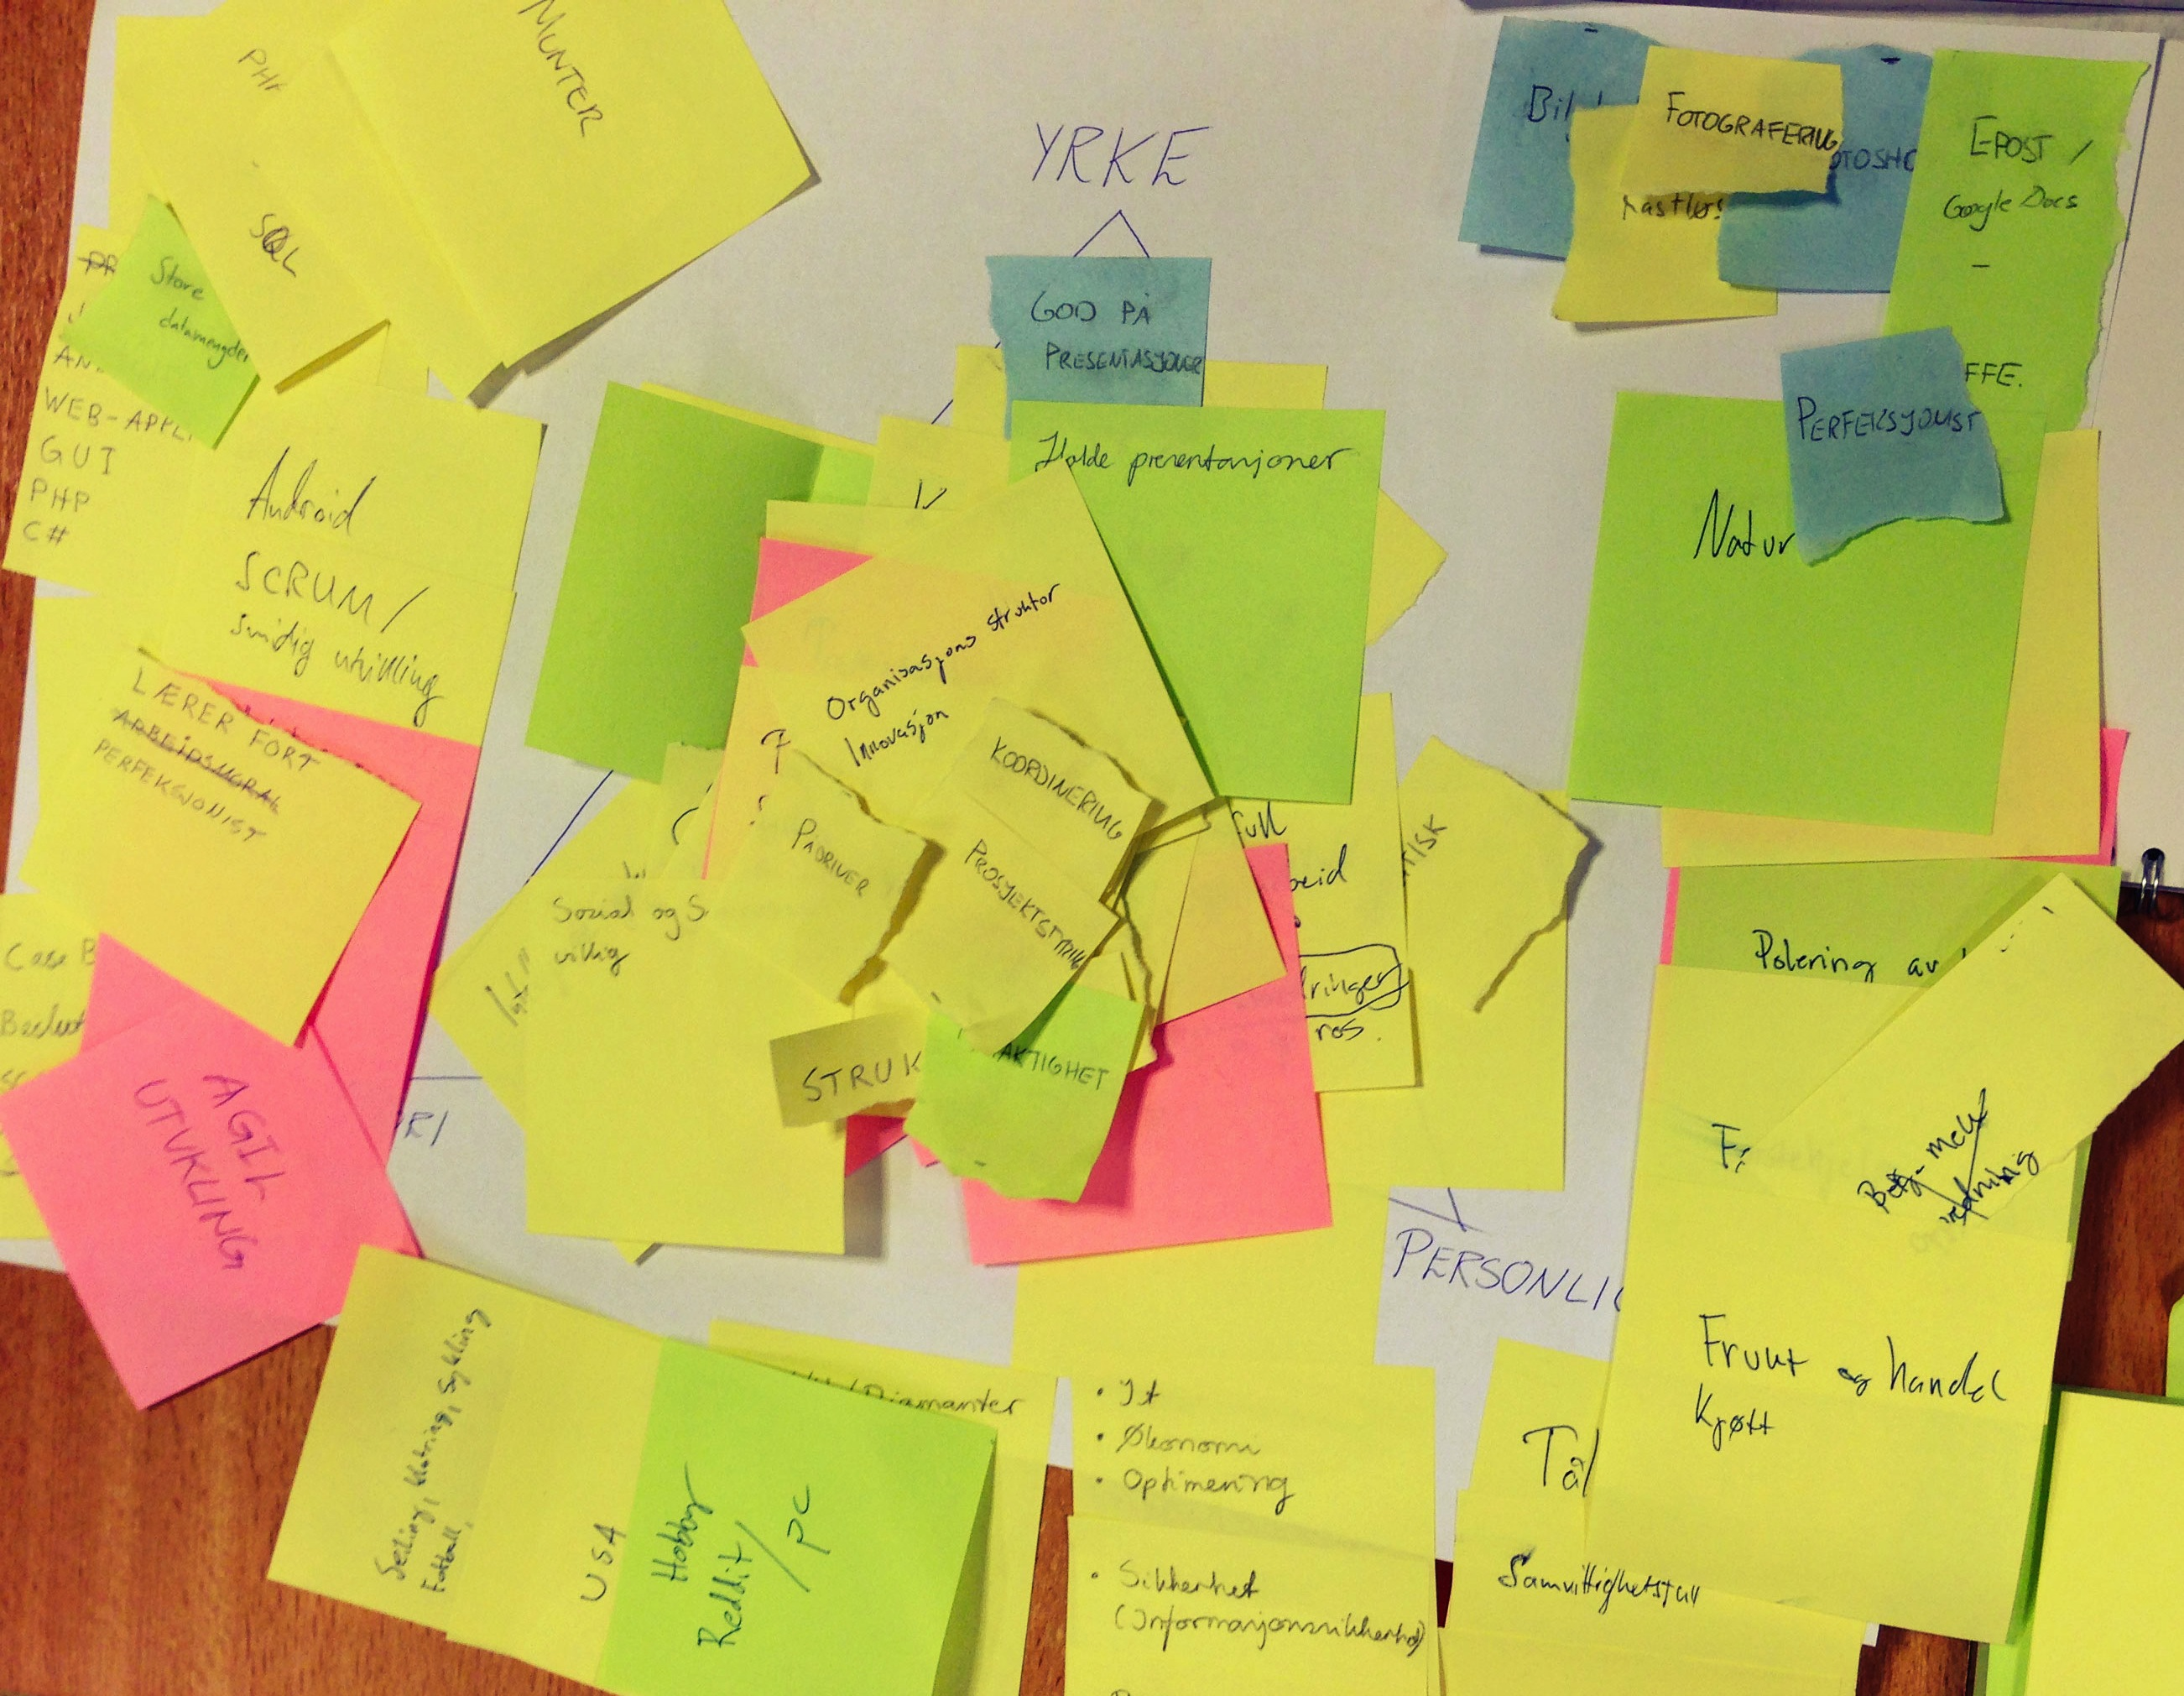
\includegraphics[scale=0.10]{figs/kompetansetrekant}
\label{kompetansetrekant}
\caption{Kompetansetrekant}
\end{figure}



Hadde vi uført denne øvelsen idag hadde vi sannsynligvis vært mer kritiske til hvilke post-it lapper som faktisk hadde vært til nytte for prosjektet. I startfasen var vi såpass forsiktige at ingen følte seg komfortable med å si ifra dersom de var uenige i relevant kompetanse. Når hver enkelt la frem sin kompetanse som han/hun mente var relevant for prosjektet, var alle automatisk enige og nikket bekreftende med hodet som en indikasjon på at personen mente det samme. Det kan ha vært tilfellet at enkelte mente at noen av post-it-lappene som ble plassert mot midten var irelevante, men ikke var modige nok til å si ifra om dette.  

\subsubsection{Storming}
I storming-fasen vil forskjellige ideer og tanker konkurrere om aksept. Gruppen diskuterer gjerne hva som faktisk er problemet som skal løses og hvilken lederskapsmodell gruppen skal følge. Det er i denne fasen gruppens medlemmer vil begynne å utfordre hverandre og det kan være en vanskelig fase for konfliktsky medlemmer. Det er også en viktig fase for gruppen som avgjør hvordan gruppen vil fungere videre. Denne fasen kan være fort overstått hvis det er høy grad av modenhet blant gruppemedlemmer. Noen grupper kommer aldri forbi denne fasen.

Idémyldringsfasen til gruppen vår var preget av å sitte fast i forming-fasen helt til eksterne tidsfrister presset oss til å forkaste problemstillinger og komme til enighet om en problemstilling. 

Overgangene mellom faser vil alltid være flytende i en gruppeutviklingsprosess og det er vanskelig å stadfeste et nøyaktig skille. Det klareste skillet for vår del kom da vi ble nødt til å formulere et prosjektforslag og med dette ble tvunget til å snevre inn ideene vi hadde diskutert og forkaste de ideene vi ikke ville jobbe videre med. Sania var fraværende under andre idémyldring og hadde fattet interesse for en annen idé enn den resten av gruppen hadde samlet seg rundt, men befant seg fortsatt til en viss grad i forming-fasen og var ikke villig til å utfordre de andre i stor grad fordi hun var redd for å være uenig meg gruppen og på den måten bli utstøtt eller miste aksept. Hun måtte derfor gi avkall på sin idé for at gruppen skulle kunne komme seg over i norming-fasen.

27.02 hadde gruppen fått i oppgave å presentere en del av pensummet i EiT for de andre i klassen. Gruppen opplevde at oppgaven kom litt brått og måtte sette til side det planlagte arbeidet med prosjektdelen for å jobbe med dette. Gruppen diskuterte innledningsvis hvordan vi skulle organisere presentasjonen og Odd Andreas luftet idéen om å bruke et mer avansert presentasjonsverktøy, slik at han fikk mer erfaring med verktøyet til ITS-presentasjonen. Diskusjonen som fulgte gjorde at Øystein kom med følgende direkte kommentar “det er vel ikke noe vits i å bruke så mye tid på presentasjonen?” Dette begrunnet han med at kvaliteten av presentasjonen ikke er en del av vurderingsgrunnlaget og implisitt mente at vi ikke skulle bruke dyrebar tid på et sidespor av prosjektet. Gruppen ble litt satt ut, men gikk videre med arbeidet. Gruppen brøt med dette en av grunnreglene for effektivt gruppearbeid som er fastslått i \cite{schwarz}. Grunnreglen sier at man skal teste antagelser og slutninger som blir gjort. I følge Schwarz er det 6 trinn i å teste antagelser og slutninger:

Observere adferd
Trekke slutninger om hva som menes
Ta en beslutning på om man bør teste slutningen som er trukket
Beskrive adferden for de andre og se hva slags slutninger de trekker
Del din egen oppfattelse med de andre
Be de andre teste sine slutninger om nødvendig.

Bakgrunnen for at det kan være nødvendig å teste antagelser er at alle oversetter observerbar data til informasjon på forskjellige måter etter hvordan de oppfatter situasjonen. Her spiller fordommer, tidligere antagelser og humør inn. Det er med dette lett å trekke feil slutninger som kan være ødeleggende for samarbeidet. I dette tilfellet var det først da vi skrev gruppelogg senere på dagen at vi reflekterte over uttalelsen og det viste seg at alle i gruppen satt med et forskjellig inntrykk av hva Øystein hadde ment.

I diskusjonen som ble gjort under skrivingen av gruppeloggen ble det klart at Steffen reagerte på utsagnet fordi han følte at Øystein ikke begrunnet hans synspunkt godt nok. Steffen savnet en utbrodering, og tok utsagnet som om Øystein ikke var interessert i å jobbe med oppgaven i det hele tatt. Sania viste gjennom sitt kroppspråk at hun var uenig i synspunktet, noe alle andre på gruppen senere ga uttrykk for at de registrerte. Allikevel fremmet hun ikke sitt synspunkt. Hun visste ikke helt hva hun skulle si, fordi hun hadde ikke vurderingen i bakhodet, men ønsket å fremføre en god presentasjon. Odd Andreas følte at gruppen ikke var så imøtekommende til hans forslag, men hadde en forståelse for at vi var under tidspress. I tillegg var det ikke en idé han ikke hadde et sterkt forhold til og derfor ikke argumenterte sterkt for.

Dette er en typisk misforståelse som kan oppstå som følge av mangelfull kommunikasjon mellom gruppemedlemmene. Øystein kommuniserte sitt syn på en veldig bastant måte, som ga lite rom for diskusjon i ettertid. Alle de andre gjorde sine egne, litt forskjellige antagelser om hva Øystein mente med utsagnet, men det ble ikke gjort noen innsats for å prøve å få klarhet i om antagelsene stemte. Når vi ser på trinnene for testing av antakelser, ser vi at gruppen ikke beveget seg over i de tre siste stegene, der man begrunner sine synspunkt og forklarer sine hensikter.

Alle i gruppen registrerte også Sania sitt kroppsspråk, allikevel var det ingen som valgte å konfrontere det. Noe kan forklares ved at Øystein senere delvis forklarte sitt synspunkt og at gruppen stort sett var enige, men det er fremdeles betenkelig at ingen i gruppen sa i fra med en gang om hvordan de reagerte på utsagnet. Flere av gruppemedlemmene ga i etterkant uttrykk for at de var veldig fokusert på målet om å sluttføre presentasjonen. Dette kan være en av grunnene til at ingenting ble sagt, vi var for fokuserte på det endelige målet om å fullføre presentasjonen og mindre opptatt av prosessen til å registrere at vi faktisk hadde en konflikt. Når gruppeloggen ble tatt opp ble vi oppmerksomme på de ulike meningene rundt denne situasjonen. Det kan argumenters for at vi i denne situasjonen befinner vi oss i den nedre delen av gruppeytelse diagrammet. Før refleksjonen hadde vi et inntrykk om at gruppen vår hadde en god dynamikk med god kommunikasjon. Refleksjonen i ettertid klargjorde at dette ikke var tilfelle og at vi hadde en del problemer, blant annet det å ta i bruk testing av antagleser. Som kjennetegner høyere effektivitetsgrupper.

Etter refleksjonen rundt situasjonen ble vi enige om at vi måtte bli flinkere på å dele og forklare vårt syn rundt saker, selv om man ikke er enige med det som blir sagt. Det ble klart at vi var nødt til å fulllføre syklusen for testing av antagelser og gjennomføre de tre siste stegene. 

Det må poengteres at gruppen vår har hoppet litt opp og ned i ytelsesdiagrammet som omhandler gruppedynamikk. Spesielt kan det nevnes fra Gruppelogg 13/03 hvor vi tydelig går gjennom en lignende situasjon, men hvor antakelser blir testet og utfallet blir et annet, oppgaven blir mer konkretisert mellom gruppemedlemmene. 

\subsubsection{Norming}
I norming-fasen har gruppen blitt enig om en felles strategi og et felles mål. Dette innebærer ofte at noen må ha gitt avkall på sine egne ideer. Gruppen går her over i en “perfoming stage” \cite{johnson2008joining} hvor rolleinndeling og ansvar blir mer tydelig mellom gruppemedlemmene og produksjon blir satt i høysetet. Enkeltmedlemmene av gruppen står nå til ansvar for gruppens suksess.

Etter å ha formulert en samarbeidsavtale og bestemt oss for prosjekt er det naturlig å regne at vi hadde kommet oss over i normings-fasen. Gruppen hadde tydlig modnet og enkeltmedlemmer tok selv initiativ til arbeidsoppgaver og samarbeid i denne delen av prosjektet. Det er også gjennomgående at kommunikasjon mellom medlemmene ble mer prosjektrettet, istedenfor der vi tidligere kunne finne på å spore av i samtalene. Dette er også et kjennetegn for normeringsfasen hvor gruppenormer, rolleinndeling og passende oppførsel er blitt forstått og godtatt av gruppemedlemmene. Mye av dette kom som naturlig utvikling på grunn av samarbeidsavtalen. Det var her at fasiliteringen og prosessrapporten ble sett som en ekstra byrde av gruppen, siden vi nå var inne i en periode man ville produsere men fikk stadige nye arbeidsoppgavere som måtte vektlegges. 

I tiden før presentasjonen hadde gruppen det hektisk med både prosjekt- og prosessrapport. Gruppen ble enige om at Steffen skulle presentere på vegne av gruppen da han hadde kompetanse på dette, og på denne måten frigjøre andre til å jobbe med rapportene. Denne avgjørelsen ble tatt raskt, og uten stor diskusjon, men med konsensus. Dette viser at vi har modnet siden første landsbydag, og nå er i stand til å ta raskere avgjørelser da tilliten er større og vi kjenner hverandre bedre.

Etter hvert som gruppen kom godt i gang med prosjektrapporten, og dokumentene var på god vei mot ferdigstillelse, ble det mindre av gjenstående arbeid. Sania følte at hun ikke hadde noe særlig mer å bidra til i prosjektdelen, og begynte å arbeide med prosessdelen av faget. Hun føler ikke at hun ville tatt initiativ på denne måten tidligere, men følte seg nå mer komfortabel med å ta avgjørelser på egen hånd. Dette tolker vi som et tegn på at gruppen hadde utviklet seg til et punkt der Sania var trygg nok på seg selv og sin plass i gruppen til å ta ansvar for denne delen av prosjektet. Dette var typisk for samtlige gruppemedlemmer på dette stadiet, alle sto frem og tok ansvar. 

\section{Personlig utvikling for gruppemedlemmene}

I tillegg til at gruppen som helhet har utviklet seg i løpet av prosjektet har vi også observert endringer i hvordan hver enkelt gruppemedlem har oppført seg. “Eksperter i Team” har et stort fokus på relasjoner, og viktigheten av å bli kjent med hverandre. I løpet av prosjektet har vi gjennomført mange øvelser som skulle hjelpe oss i å identifisere roller, kompetanse og personlige egneskaper. Deriblant den overnevnte kompetansetrekanten, legoøvelsen, The Marsmallow Challenge og SPGR. Selv om disse øvelsene var nyttige på sin egen måte, var det SPGR testen gruppen følte vi fikk mest ut av, spesielt med tanke på å avdekke endringer i hver enkelt persons atferd i gruppen. Det faktum at vi gjennomførte testen to ganger gav oss en håndfast måte å måle endringer i både gruppen og hos enkeltpersoner. Derfor har vi valgt å se nærmere på resultatene fra disse testene.
	
\subsection{SPGR}
SPGR-øvelsen er basert på modellen til Endre Sjøvold.\cite{endre} Øvelsen omhandler å kunne reflektere rundt egne handlingmønstre og egen atferd. Øvelsen er situasjonsbetinget, det betyr at resultatet varierer fra situasjon til situasjon. For å understreke dette bruker Sjøvold funksjoner fremfor roller, da roller er mer statiske. I tillegg til å reflektere over seg selv, egen oppførsel og handlinger, skal også andres væremåte analyseres, for så å tas opp i plenum. 

Figuren er delt i tre deler, hvor hver del kjennetegnes med en bestemt farge. Blått signaliserer kontroll, grønt står for omsorg, mens opprør har fått tildelt en rød farge. SPGR-testen ble utført to ganger, den første gangen ganske tidlig i prosessen, mens andre gangen ble den utført mot slutten av arbeidet. 


\begin{figure}[H]
\centering
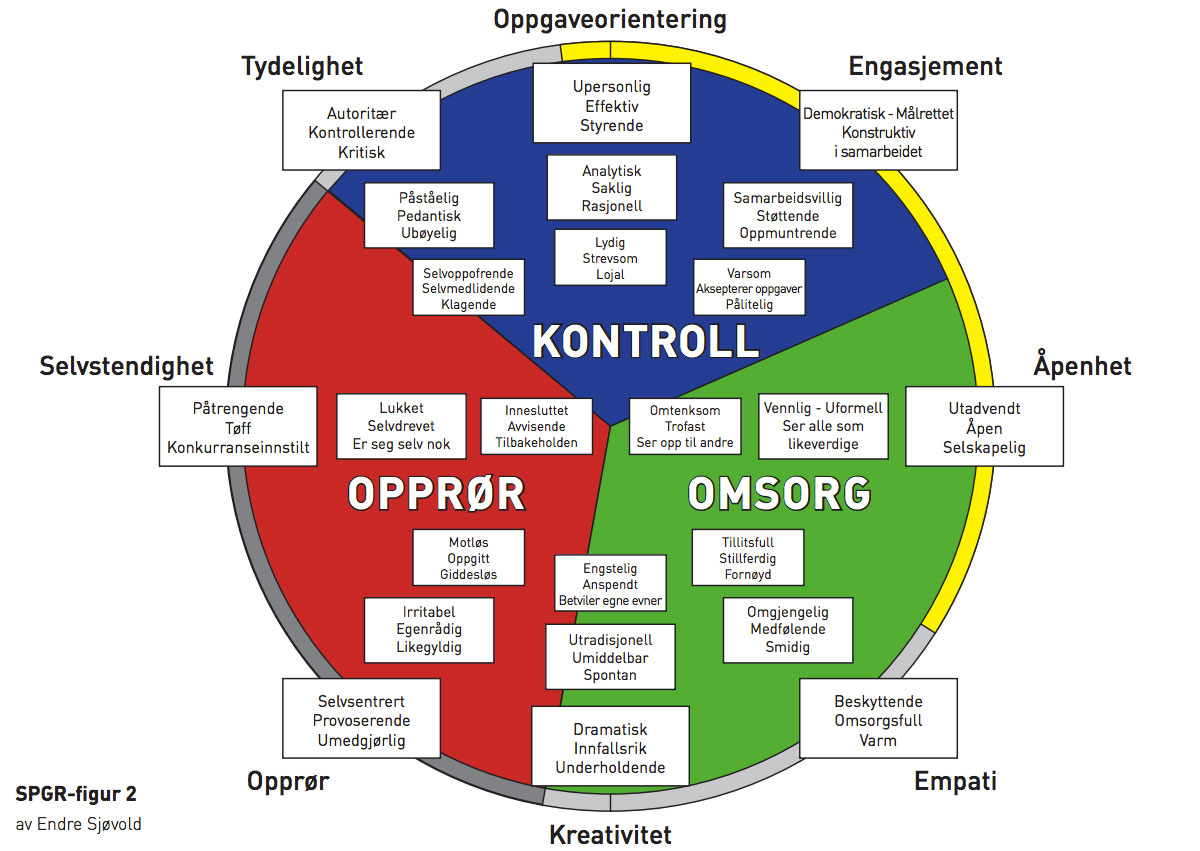
\includegraphics[scale=0.25]{figs/spgrfigur2}
\label{spgr}
\caption{SPGR-rommet slik det er definert av Endre Sjøvold}
\end{figure}

\clearpage




\subsubsection{SPGR-test 06.02.2013}
Det første testen ble gjennomført tidlig i prosjektet. 

De andre på gruppen beskrev Øystein som litt innesluttet i begynnelsen. Han ble oppfattet som veldig saklig og analytisk i diskusjoner, men kunne bli flinkere til å fremme sine synspunkter oftere. De andre mente alikevel at Øystein var en person som hadde mye å tilføre gruppen. Øystein selv var ikke spesielt overrasket over tilbakemeldingene. Mye av det som kom frem var som forventet. Han er vant til å få slike tilbakemeldinger fra andre, spesielt fra personer han ikke er så godt kjent med.

Tilbakemeldingene Odd Andreas fikk gikk i stor grad ut på at han hadde mange idéer om hvordan ting kunne løses, men ofte ikke kjempet nok for å få gjennomslag for sine egne idéer.
Odd Andreas sa selv at han ofte betviler egne evner. Siden han har lite erfaring med gruppearbeid på NTNU og ikke har hatt mye tid til å bygge et sosialt nettverk er han ofte usikker på hvor mye kunnskap han sitter på i forhold til de andre. I dette gruppeoppsettet kan dette være et ekstra stort problem, ettersom gruppen har to andre fra samme studieretning. Gruppen hadde lagt merke til dette og kommenterte at de følte han var litt usikker, men hadde tro på at han ville gjøre en bedre jobb enn han selv trodde.

Steffen gikk skeptisk til den første SPGR-testen. Han syntes det var vanskelig å få tak på formålet med testen før vi satte igang og merket liten motivasjon. Dette endret seg relativt raskt etter at testen hadde begynt. Steffen fikk nesten utelukkende positive tilbakemeldinger. Det kan være at gruppe ikke turde å være hundre prosent ærlig siden han var den første som ble diskutert. Steffen er gruppens koordinator og fikk tilbakemeldinger om at gruppemedlemmene savnet en hardere hånd og mer gjennomslagskraft. Koordinatorrollen er en rolle han ikke har hatt i tidligere grupper.

Sania ble beskrevet som en blid og samarbeidsvillig person. Hun var flink til å oppmuntre og gi positive tilbakemeldinger til de andre på gruppen. For atferd brukt konstruktivt ble hun markert som pålitelig, strevsom, utadvendt og vennlig. Gruppen ønsket imdilertid å se mer av Sanias tøffe side. Gruppen mente at hun under avgjørelsen om valg av prosjektoppgave gav veldig fort etter og ikke sto fast ved at hun ønsket en annen formulering på oppgaven. De hadde også opplevd i en rekke situasjoner at hun kanskje nølte med å si ifra dersom hun var uenig i noe som ble sagt eller gjort. 

Eirik fikk tilbakemelding om at han var en kreativ og en humørfylt person som var lett å snakke med. Adferd som de andre hadde bemerket seg var at han var tidlig ute med idéer. Han viste et engasjement for EiT med tydlighet, åpenhet, kreativitet og empati som gjengangere i tilbakemeldingene. Plasseringen i SPGR-rommet var tydelig på omsorgsiden. Adferd de ville se mer av var opprørskhet og mer oppgaveorientering. 

Andreas ble beskrevet som hyggelig og morsom, men også som reflektert og saklig. Steffen uttrykte at han på en positiv måte syntes Andreas var vanskelig å plassere. Mange hadde krysset av for atferd vi ser og vil se mer av på analytisk, saklig, rasjonell og samarbeidsvillig, støttende, oppmuntrende.


Utbyttet gruppen fikk av SPGR-testen økte da vi valgte å snakke løst rundt temaene i figuren, uten å følge systemet slavisk. På den måten ble praten mer åpen, innspillene baserte seg oftere på konkrete situasjoner og diskusjonen ble oppfattet som mer ærlig og direkte. 

Gruppen som en helhet plasserte seg i sonen som betegner engasjement og oppgaveorientering. Den røde sonen som representerer selvstendighet og opprørskhet lå gruppen langt unna. Dette tyder på at gruppen er i formingfasen, og gruppemedlemmene hadde fokus på å unngå konflikter. Tilbakemeldingene i testen var farget av dette, og inneholdt lite kritikk. Det kan også være at grunnlaget vi vurderte hverandre på i den første testen er så tynt at vi ikke hadde sett nok til å kunne gi en nøyaktig tilbakemelding. Alle gruppemedlemmene var enige om at vi ikke var opprørske, og tøffe nok til å si ifra om noe man reagerte på. Vi ble enige om å forsøke å tørre å si ifra selvom det kunne skape en konflikt. 

En gjennomgående trend var at de fleste tilbakemeldingene ikke var overraskende for gruppens medlemmer. Medlemmene syntes dog at det var svært positivt med en så konkret tilbakemelding, og at SPGR-testen åpnet for en mer åpen og ærlig arena for diskusjon om gruppearbeidet i gruppen. Tilbakemeldingene gav også mulighet til å identifisere områder man kunne bli bedre på.


\subsubsection{SPGR-test 06.04.2013}
Det siste SPGR testen ble gjennomført mot slutten av prosjektet.

Øystein selv følte at han hadde blitt mer åpen og utadvent siden forrige test, og det stemte godt overens med tilbakemeldingene fra resten av gruppen. Etter den forrige SPGR-testen ble det fokusert på at Øystein kunne være flinkere til å si ifra når han hadde noe å komme med og det var bred enighet om at han har tatt tak i dette. Han blir oppfattet som en effektiv og pålitelig person som fullfører de oppgavene han får tildelt. Resten av gruppen syntes han var en av dem som hadde forandret seg mest fra den første testen.
Odd Andreas følte ikke han hadde forandret seg mye. Det var fortsatt tilbakemeldinger som gikk på at han var litt lite bastant og tøff, men Eirik og Andreas hadde lagt merke at han var flinkere på dette når de hadde jobbet sammen på tomannshånd. Odd Andreas betvilte fortsatt sine egne evner. Gruppemedlemmene beskrev han som pålitelig og arbeidssom, selvom han selv så på seg selv mer som en humørspreder. I denne testen plasserer Odd Andreas seg mer mot tydelighet og selvstendighet enn i den første testen. Han har ikke beveget seg spesielt langt på diagrammet, men oppfattes som litt tøffere, spesielt når han forholder seg til enkeltpersoner.
Den andre SPGR-testen var ikke ulik den første. Tilbakemeldingene var stort sett de samme og pekte i kun små endringer for Steffen. Gruppen mente at Steffen som koordinator kunne vært enda tydeligere. Steffen har vært syk ved to anledninger dette semesteret og har med dette mistet noe av oversikten over prosjektet. Da ble det vanskelig å koordinere arbeid og samkjøre gruppen. Dette følte også gruppen og gav han tilbakemelding på dette under SPGR-testen.
Sania hadde tatt til seg det som ble sagt tidligere om å bli mer påtrengende og tøff. De hadde merket at hun hadde sluppet seg litt mer løs og begynt å tørre i si ifra. Denne gangen hadde Sania også fått et mer autoritært og kontrollerende preg, noe som ikke var synlig før. Gruppen som helhet syns det var positivt å se denne siden av henne. Påtrengde og tøff var nå i en mer grønn sone (som før var i en gul).
Eirik lå fortsatt på omsorgssiden, men fikk tilbakemelding om at han var litt mer opprørsk av seg men fortsatt hadde en del å gå på. Tilbakemeldingen fra den første SPGR-testen til denne var fortsatt rimlig lik noe Eirik syntes var uheldig. Noe av grunnen for dette kan være at han meldte seg ut av gruppearbeidet i det gruppen startet å klargjøre for ITS-konferansen. Da han ikke ville ha anledning til å være med på framføringen ble det mer naturlig å la andre ta seg av hva som skulle framføres, siden han dro ut av landet i en lengre periode. Hadde han ikke vært fraværende mente han at han ville bli ansett som mer oppgaveorientert og opprørsk person siden han ved forrige SPGR-test fikk tilbakemelding om at dette var noe han måtte jobbe med. 
Steffen syntes Andreas var den som hadde flyttet minst på seg i SPGR-diagrammet og det var bred enighet rundt dette. Andreas mente at dette kunne være fordi han i starten av prosjektet bevisst hadde gått inn for å være seg selv uten å holde igjen for mye. Samtidig mente Sania at Andreas hadde lukket seg litt og var litt mer tilbakeholden, men at hun trodde det hadde sammenheng med et hektisk studieliv som tilspisser seg med mange innleveringer i det tidsrommet den andre SPGR-testen ble gjennomført og at det kunne være bakgrunnen for dette.

Vi følte det var enklere å gjennomføre den andre testen. Vi hadde gjort det en gang før, dermed visste alle hva de gikk til. I tillegg var det nå enklere å knytte egenskaper opp mot spesifike situasjoner, da vi hadde jobbet sammen over en lengre periode. En klar trend i denne testen var at det var lite avvik i tilbakemeldingene medlemmene fikk. Det var også større samsvar mellom måten folk karakteriserte seg selv og måten andre karakteriserte dem. Dette er kanskje et tegn på at vi har klart å skape klare forventninger til gruppens medlemmer, slik at de klarer å plassere seg selv og rollen de spiller i gruppen mer nøyaktig.

Generelt sett har ikke medlemmene i gruppen gjennomgått store endringer, noe som stemmer overens med det vi ble fortalt om utviklingen i EiT-grupper i en videoforelesning. Men enkelte har vært flinke til å forsterke atferd som har vært ønsket av de andre medlemmene i gruppen. Øystein har vært flink til å være mer utadvent og åpen. Etter den forrige SPGR-testen ble det fokusert på at Øystein kunne være flinkere til å si ifra når han hadde noe å komme med og det var bred enighet om at han har tatt tak i dette. Det ble også fokusert på at Sania godt kunne kjempe hardere for meningene sine og ta mer kontroll. Dette har hun tatt til seg og har vært dyktig til å sørge for at hun blir hørt. Begge er eksempler på at SPGR testen har hjulpet oss i å identifisere forbedringspotensialer, og at gruppens medlemmer tok tilbakemeldingene til seg. Alle i gruppen har siden første SPGR-test blitt flinkere til å konfontrere og si ifra. Vi beveget oss mer mot den opprørske siden, og ser at tilbakemeldingene fra SPGR-tester endrer gruppedynamikken. Dette kan tolkes som et tegn på at gruppens medlemmer var åpen til prosessdelen av faget. Samtlige var åpen for kritikk og tok dette til seg med et ønske om å forbedre seg.

\section{Hva hver enkelt fikk ut av emnet}

\subsection{Steffen}
Steffen har lært mye om å lede en gruppe gjennom rollen som gruppens koordinator. Dette er en rolle han ikke var vant med fra før, men som han tok på seg for å lære mer om. Gjennom SPGR-testene fikk han tilbakemelding om å bli tøffere, bruke større gjennomslagskraft og være en sterkere leder. Dette overrasket Steffen, og han har lært at gruppemedlemmer liker å bli ledet. Og at man som en god leder må ta skikkelig kontroll. Lenge forsøkte Steffen å kun bruke sin koordinatorrolle der han så behov for det, men etter tilbakemeldinger fra gruppen forsøkte han å bli tøffere uten å lyktes. Han fikk tilbakemeldinger om å være enda mer tøff. Han merket også at han etter en sykdomsperiode hadde problemer med å koordinere gruppen da han ikke hadde oversikt. På den måten erfarte han at en gruppeleder må ha full oversikt over hva gruppen holder på med for å fordele arbeid på en god måte.
Videre har han lært at gruppesamarbeid er en ferdighet som kan læres. Han har gjenkjent “bli-kjent-fasen” i tidligere gruppesamarbeid og sett at erfarne gruppemedlemmer bruker kortere tid i denne fasen, og beveger seg over i mer effektive faser på et tidligere stadie. Han har også lært øvelsen “The Marshmallow Challenge” som han har lyst til å bruke i Fotogjengen på Samfundet i et forsøk på å belyse gruppesamarbeid.

\subsection{Øystein} 
Øystein hadde ikke særlig store forventninger til faget når prosjektet begynte, men føler han sitter igjen med overraskende mye. En av de viktigste tingene han har lært er viktigheten av å tidlig stille klare forventninger til hverandre innad i gruppen. Ved å tidlig avklare hva hver enkelt forventer å få ut i fra prosjektet opplevde han det som enklere å forholde seg til de andre på gruppen og enklere å komme frem til et felles mål. 

Han opplevde det også spesielt nyttig med åpenheten rundt prosessen, noe som var veldig annerledes fra andre gruppearbeid. I begynnelsen oppfattet han prosessdelen som unødvendig og lite interessant, men har etterhvert lært å sette pris på den. Han har erfart i dette prosjektet hvor nyttig det faktisk er og hvor mye det har å si for resultatet av gruppearbeidet. Spesielt det å evaluere både sin egen innsats og gruppen som helhet jevnlig er noe han ikke har gjort ved tidligere anledninger. Slike aktiviteter har vært med på å skape en åpen arena der man kan lufte frustrasjoner og håndtere dem før det får ødeleggende konsekvenser for gruppen. Det har også vært nyttig for å identifisere områder han selv kan bli bedre på.

Han har i tillegg opplevd at det er viktig med kunnskap om teori bak gruppedynamikk for å bli god på gruppearbeid. Han har kjent seg igjen i overraskende mange av de situasjonene som er beskrevet i pensum fra tidligere prosjektarbeid, og kan nå peke på elementer som bidro til at ikke alt gikk på skinner den gang. Med forståelse for teorien kan han i fremtiden identifisere slike situasjonene tidlig og håndtere dem på en god måte.

\subsection{Odd} 
Odd Andreas har ikke hatt mange tidligere erfaringer fra gruppearbeid, og erfaringene har sjelden vært gode da de generelt bare har vært gruppearbeid på et “pseudonivå”, hvor gruppemedlemmene i større grad føler at de konkurrerer med hverandre. At EiT fokuserer på selve prosessen rundt gruppearbeidet har hjulpet han med å bli mer oppmerksom på nyttige tiltak som han kan ta med videre.
Det viktigste han har lært er hvor viktig det er å ikke bare ‘være ærlig’ med sine gruppemedlemmer, men hvor viktig det er å sette av en tid hvor man oppmuntrer til ærlighet. Det å bestemme seg for å være mer ærlig er vanskelig, og kan gjøres lettere dersom man skaper et miljø for det. Et eksempel er gruppeloggene på slutten av dagen, som har gjort en god jobb med å grave frem relativt irrelevante problemer og små irritasjoner som kunne ha vokst til å bli store konflikter over tid. SPGR-testene har også vært gode eksempler på situasjoner som oppmuntrer til ærlighet. Han har også lært at det viktigste ikke nødvendigvis er å bestemme seg for at man skal være ærlig og åpen selv, men at man gjør det klart at man syns det er greit at andre er ærlige og åpne, og at man er interessert i å få slike tilbakemeldinger. Fasilitatorene snakket ofte om at det å kritisere andre sitt arbeid ikke bør oppleves som negativt, men at det tvert imot hjelper dem med å bli mer sikre på kvaliteten i det de produserer. Odd Andreas var enig i dette, men var alikevel usikker på om andre følte det samme eller om de ville oppfatte kritikk som utelukkende negativt og demoraliserende. Underveis i prosjektet gjorde Øystein det klart at han foretrakk kritisk tilbakemelding på det han har skrevet i rapporten fremfor positive tilbakemeldinger, og dette bidro til ærligere kritikk fra Odd Andreas.
I tilbakemeldingene til Odd Andreas presiserte gruppen at de ønsket at han var mer frempå med sine meninger. Den siste SPGR-testen viser at de han jobbet med på individuelt nivå hadde opplevd at han var blitt dyktigere på dette. Han føler ikke selv at han har lært noe på dette punktet, men snarere at han har fått bedre selvtillit fordi han har arbeidet mye mer med studenter på hans nivå slik at han har fått sammenlignet seg med andre og justert forventningene til seg selv.

\subsection{Andreas}
Andreas mener at det viktigste han har lært i eksperter i team er viktigheten av å være åpen om hva som forventes av hverandre og viktigheten av å være tøffe nok til å komme med kritikk tidlig i prosessen når man mener at det som blir gjort ikke  er hensiktsmessig for gruppen. Det at man i starten av prosjektet bevisst har en diskusjon rundt hva hver enkelt ønsker å oppnå og blir enige om hva gruppen har som mål førte til at alle til enhver tid hadde et klart bilde av hva de andre forventet av dem. Dette gjør også at medlemmene føler seg mer komfortable med å si i fra når de føler at arbeidet som blir gjort ikke samsvarer med de målene gruppen har satt seg som helhet. Det er til stor hjelp at gruppen har felles referanserammer når det kommer til å diskutere om arbeidet samsvarer med de målene man har satt seg. En felles ontologi gjør at det både føles mindre ubehagelig å ta opp problemer og at noen tar opp et problem med deg. Det er lettere å diskutere atferd i forhold til forventning når man har klart definerte retningslinjer. Tilbakemeldingene føles i denne sammenhengen mindre personrettet og mer saklig. Dette gjør at kursen fort kan rettes opp når gruppen kommer på feil spor, samt at man unngår unødvendige konflikter som oppstår når noen over lang tid er misfornøyde med det som blir gjort uten å si i fra. I situasjoner hvor medlemmer av gruppen føler at forventningene ikke blir møtt uten å si i fra om dette kan det føre til unødvendig irritasjon. Dette fører ofte til at man delvis melder seg ut av gruppen uten at det har blitt gjort noe forsøk på å løse konflikten som fører til dette. I sammenheng med dette har det også vært lærerikt å reflektere over at alle i en gruppe er ansvarlig for gruppens suksess. Når arbeidet ikke går i den retningen man vil er det lett å trekke seg ut av gruppen og konstatere at det er de andre i gruppen som er årsaken til problemene, uten å innse at man ved å unngå å forsøke å løse et problem som oppstår et annet sted i gruppen fraskriver seg det ansvaret man har for gruppens suksess som helhet. Dette er riktignok en erfaring som springer ut fra å koble teori fra EiT-pensum med gruppearbeid i andre fag hvor samarbeidet har vært mindre vellykket, men også fra at at Andreas trakk seg litt tilbake halvveis ut i lego-øvelsen da han mente at gruppen ikke var på rett spor, men ikke gjorde noe for å komme med innspill.  

\subsection{Sania}
Sania har vært mye borti gruppearbeid under sine år på NTNU, hvor flertallet ikke har vært så altfor bra. Hun har blant annet opplevd mye skeiv fordeling av arbeid. Hun gikk med en innstilling og et håp om at dette gruppearbeidet skulle bli en bra og lærerik opplevelse. 

Det å samarbeide med individer som har en annen kompetanse enn en selv har gjort henne bevisst på viktigheten av å ta alles meninger og tanker i betraktning. Men også evnen til å kunne si ifra og være litt tøff har blitt satt på prøve. Sania er ikke alltid like flink å si ifra dersom hun er uenig i noe gruppen tar for seg.  Under øvelsene i faget, samt ved hjelp av samtaler og diskusjoner, ble hun bevisst på at hun burde bli litt tøffere og kritisk. Ikke minst at det ikke er farlig å sette ned foten hvis man ønsker å gjøre noe på en annen måte en alle andre. Det var først under SPGR-testen dette ble understreket av de andre på gruppen. Det var egentlig litt godt for henne å høre at andre ønsker å se henne tøffere, for da gikk hun inn for å være litt mer frempå. Hadde ikke denne tilbakemeldingen vært i bildet, ville hun sannsynligvis ha fortsatt å være tilbakeholden. 
Det har også vært meget lærerikt å jobbe i et tverrfaglig team. Det er i den slags samarbeid essensiellt å lytte til hverandre og la hver enkelt få si sin mening. Det kan oppstå situasjoner hvor man ikke forstår begreper og uttrykk relatert til andre fagfelt, og det er da viktig å spørre. Ikke minst er det viktig at den som snakker er bevisst på at det andre på gruppen som muligens ikke har hørt om det som for deg kan være selvforklarende.     

\subsection{Eirik}
Det å “teste sine antagelser” har vist seg at øker kommunikasjon mellom gruppemedlemmene og er et enkelt virkemiddel i gruppearbeid, som minker stressmomenter og feilkilder i arbeidet. Eksperter i team gir deg en praktisk og teoretisk forståelse av hva gruppearbeid innebærer. Det å kunne reflektere og analysere forskjellige hendelser som en gruppe har vært i, for så å kjenne seg igjen i litteraturen er noe Eirik aldri har gjort tidligere med tanke på gruppearbeid. Hvordan de ulike gruppene kan differensieres og hvordan målsette dette med tanke på diagrammet for en lukket gruppe versus en åpen gruppe. At en åpen eller lukket gruppe ikke alltid er svaret for en gitt problem, men at høy produktivitetsgrupper ofte har en åpen gruppestruktur hvor hvem som er lederen er vanskelig å definere. Emnet har også gitt han forståelse for at en klar visjon og målsetning er viktig fordi man tidlig i fasen kan fastsette de ulike forventningene man har til de ulike deltakerne av gruppen, og at det er her samarbeidsavtalen blir et viktig poeng. For om det skulle komme til uenigheter er det kjekt om man kan bruke samarbeidsavtalen til å holde konflikten nøytral ved å påpeke tidligere fastsatte krav og ikke synsing som kan oppfattes som subjektiv, uformel og partisk. Personlig har han lært hvordan andre oppfatter han og hvordan han supplerer gruppen på godt og ondt spesielt ble dette tydlig under SPGR-testen. I en gruppe med mange fagdisipliner og forskjellige bakgrunner, hvordan kan man gi konstruktiv kritikk på ting man ikke nødvendigvis er ekspert på? 

\section{Fasiliteringen}
Fasiliteringen skal være til hjelp for studentene for refleksjon, samt gi tilbakemeldinger relatert til blant annet gruppeloggene. I vår landsby var det to studentassistenter som fungerte som fasililatorer. 

Gruppen sitter igjen med  blandede opplevelser av fasiliteringen og dens funksjon. Tilbakemeldingen etter hver enkelt gruppelogg har vært til stor nytte for oss, og gruppeloggene har også utviklet seg kraftig fra uke til uke. Fasilieringen satte ofte i gang dype diskusjoner og tankeprosesser innad i gruppen, og studentassistentene hadde ofte mange gode tips til hvordan vi kunne reflektere enda dypere. 

Da fasillitatorene skulle avlytte samtaler i gruppen brukte de ulike teknikker. En av disse var å sette seg ned med gruppen, lytte nøye på det vi sa og analysere det vi gjorde før å komme med konstruktiv og god kritikk. Denne formen for fasilitering likte vi godt, og hadde stort utbytte av. Vi syns for eksempel at sosiogrammet var en meget interessant måte å kartlegge hvordan samalene gikk i gruppen, og hvem som snakket mest/minst.  En annen teknikk som ble brukt var å avlytte uten at gruppen skulle merke at de var der. Dette ble gjort med ryggen til, og med intensjon om å være diskré uten å faktisk være det. Gruppen syntes dette var litt rart, og likte bedre når de satt seg ned med oss.  

\section{Oppsummering}
Underveis i prosjektet har gruppen ofte fokusert på temaet konfliktskyhet, og det har vært en gjenganger i de fleste gruppeloggene våre. Det har derfor også vært noe vi har jobbet mye med, og har forsøkt å løse problemet ved å gi uttrykk for at vi forventer ærlig tilbakemelding av andre gruppemedlemmer. Resultatet er at vi har sett stadige forbedringer på dette området over tid. Vi tør nå etter en modningsperiode å konfontrere andre gruppemedlemmer, og være mer opprørske og kritiske.

Etter å ha hatt emnet “Eksperter i Team” sitter vi igjen med en positiv holdning til faget. Vi har lært mye om det å jobbe i en tverrfaglig gruppe. Deriblant åpenhet, ærlighet, bevissthet, det å være kritisk og ikke betvile egne evner. Av øvelsene som har blitt utført i faget, er det uten tvil SPGR-testen vi føler vi har fått mest utbytte av, og resultatet og tilbakemeldingene er noe vi definitivt kan ta med oss videre ut i arbeidslivet. Den positive innstillingen gruppen har hatt til prosessdelen av faget helt fra starten bidro til at vi tok de ulike øvelsene mer på alvor.Teorien i kompendiet har lært oss å gjenkjenne fasene i et gruppearbeid, og har gjort oss mer effektive i tverrfaglige team.

%\backmatter
\clearpage
\bibliographystyle{plain}
\bibliography{prosbib}

\addcontentsline{toc}{chapter}{Referanser}
%\bibliography{bibtex/bibliography}





\end{document}
